\documentclass[a4paper,10pt]{article}
%Use article for short documents
\usepackage[T1]{fontenc}
\usepackage{parskip}
\usepackage{latexsym,amsmath,amssymb}
\usepackage[natbibapa]{apacite}
\usepackage{graphicx}
\usepackage{times}
%\usepackage{zi4}
\usepackage[a4paper,left=3cm,right=3cm,top=3cm,bottom=3cm]{geometry}
\usepackage{caption}
\usepackage{subcaption}
\usepackage[section]{placeins}
\usepackage{listings}
\usepackage[usenames, dvipsnames]{color}
\usepackage{bm}
\usepackage[retainorgcmds]{IEEEtrantools}
\usepackage{setspace}
\usepackage{multirow}
\usepackage{longtable}
\usepackage{subcaption}
\usepackage[stable]{footmisc}
\usepackage[showonlyrefs]{mathtools}
\usepackage{hyperref}
\usepackage{algorithm}
\usepackage{algorithmic}
% \usepackage[noend]{algpseudocode}


\DeclareMathOperator{\expectation}{E}

\newcommand{\euler}{\mathrm{e}}
\newcommand{\diff}{\mathrm{d}}
\newcommand{\T}{^\textup{T}}
\newcommand{\vect}[1]{\mathbf{#1}}
\newcommand{\vectGreek}[1]{\boldsymbol{#1}}
\newcommand{\matr}[1]{\mathsf{#1}}
\newcommand{\dotdotdot}{\vphantom{.}_{\cdots}}


\bibliographystyle{apacite}

\title{Summary Statistics for Approximate Bayesian Computation}
\author{Nathan Cunningham \and Sherman Ip \and Ella Kaye}

\begin{document}
\maketitle

\section{Introduction}
Approximate Bayesian computation (ABC) is a powerful tool that approximates sampling from a posterior distribution when the likelihood is intractable. ABC has found wide application in fields such as population genetics, where it is possible to simulate from models, but it is impossible, or computationally too expensive, to calculate the likelihood of the data.

In this report, we \ldots

\section{Background}
In a standard Bayesian inference, we wish to simulate from the posterior distribution

\[
\pi(\theta | y_\textrm{obs}) = \frac{p(y_\textrm{obs} | \theta) \pi(\Theta)}{p(y_\textrm{obs})},
\]
where $y_\textrm{obs}$ are our observed data and $\Theta$ a vector of parameters. However, doing so is impossible impossible when the likelihood is intractable. By accepting some approximations, it is still possible to performance Bayesian inference in such a setting. First, the full Bayesian posterior is approximated by a partial posterior distribution

\[
\pi(\theta | s_\textrm{obs}) = \frac{p(s_\textrm{obs} | \Theta) \pi(\theta)}{p(s_\textrm{obs})},
\]
where $s_\textrm{obs} = S(y_\textrm{obs})$ is a vector of summary statistics of a lower dimenion than the data. Since $\pi(\theta | s_\textrm{obs})$ is likely to be computationally intractable when $\pi(\Theta | y_\textrm{obs})$ is, a further approximation must be made. In the simplest ABC algorithm, rejection sampling, the ABC posterior distribution, $\pi_{\epsilon}(\theta | y_\textrm{obs})$, is generated by Algorithm \ref{alg:ABCrej}.

\begin{algorithm}
\caption{ABC by rejection sampling} \label{alg:ABCrej}
\begin{algorithmic}
\FOR{$i = 1,\ldots, N$}
\REPEAT
\STATE Generate $\theta'$ from the prior distribution $\pi(\cdot)$
\STATE Generate $y_i$ from the likelihood $p(\cdot | \theta')$
\UNTIL{$\rho\{S(y_i), S(y_\textrm{obs})\} \leq \epsilon$}
\STATE set $\theta_i = \theta'$
\ENDFOR
\end{algorithmic}
\end{algorithm}

The idea behind ABC in Algorithm \ref{alg:ABCrej} is that when the summary statistic $S$ is representative of the data and the tolerance $\epsilon$ is small enough, then $\pi_{\epsilon}(\theta | y_\textrm{obs}) \approx \pi(\theta | y_\textrm{obs})$.

There are three parameters that need tuning in Algorithm \ref{alg:ABCrej}: $S(\cdot)$ which gives the summary statistic, the distance measure $\rho$, and the tolerance $\epsilon$. Throughout this report, we take $\rho$ to be the Euclidean distance measure. 

When $\epsilon = 0$, the algorithm samples from the partial posterior. A toy example of this is discussed in Section \ref{sec:beta-bin}. However, when data is continuous, and in all real-world cases, we will have $\epsilon > 0$. Selecting $\epsilon$ is a trade-off; a small $\epsilon$ gives a closer approximation to the partial posterior, whilst at the same time increasing the compuational cost by lowering the acceptance rate. One option for tuning $\epsilon$ is through cross-validation. We take this approach in Section REF.

The selection of summary statistics is also crucial to the accuracy and efficiency of ABC. Again, there is a trade-off. With a large number of summary statistics, the error in the approximation of $p(\theta | y_\textrm{obs})$ by $p(\theta | s_\textrm{obs})$ is likely to be reduced, but the approximation of $p(\theta | y_\textrm{obs})$ by $p_\epsilon(\theta | y_\textrm{obs})$ is likely to be poor because of inefficiency. On the other hand, with only a few summary statistics, the second approximation should be good, but the first will be poor. We have that $\pi(\Theta | s_\textrm{obs}) = \pi(\Theta | y_\textrm{obs})$ if $s_\textrm{obs})$ is a sufficient statistic. However, in many applications, it will not be possible to find sufficient statistics. In early applications of ABC, summary statistics tended to be chosen in a fairly ad hoc manner. One more principled approach is that of best subset selection, which considers whether an additional summary statistic $s_k$ should be added to a model that already contains statistics $s_1, \ldots, s_{k-1}$. Even when implemented with a step-wise search algorithm, this approach becomes computationally unwieldy whenever $k$ is large. Moreover, it needs an additional tuning parameter to determine the threshold at which each statistic is either accepted or rejected. It is also possible that an accepted statistic actually biases approximation away from the true posterior.

Another approach to dimension reduction is semi-automatic ABC. \textbf{NATHAN ADD MORE HERE.}

There are a number of improvements that can be made to Algorithm \ref{alg:ABCrej} to correct for the distance between $S(y_i)$ and $S(y_\textrm{obs})$. One, suggested by REF BEAUMONT ET AL uses local linear regression, so that for each simulated $z$, we set 
\[
\theta_i = m(S(z)) + \eta_i
\]
where $m$ is the regression function and the $\eta_i$ are centered random variables with common variance. Instead of rejecting or accepting $\theta_i$ based on the threshold $\epsilon$, each simulation $(\theta_i, S(y_i))$ is then assigned a weight $K[\rho(S(y_i), S(y_\textrm{obs}))]$, based on a statistical kernel $K$, with higher weights given for proximity to the observation. 

\section{Beta prior, binomial likelihood} \label{sec:beta-bin}
\subsection{Method}
Suppose a parameter $\theta$ has a prior distribution such that
\begin{equation}
\theta\sim\textup{Beta}(1,1)
\end{equation}
and that a random variable $X$ is distributed such that
\begin{equation}
X|\theta\sim\textup{Bin}(12,\theta) \ .
\end{equation}
Then after observing $X=2$, the posterior distribution is given as
\begin{equation}
(\theta|X=2)\sim\textup{Beta}(3,11) \ .
\end{equation}
ABC was used to sample the posterior distribution where the algorithm is as followed:
\begin{itemize}
  \item Sample $\theta$ from the uniform distribution
  \item Sample $X|\theta$ from the likelihood
  \item If the sampled $X|\theta$ is equal to 2, accept $\theta$, otherwise reject.
\end{itemize}

\subsection{Results}
10,000 posterior samples were drawn from the ABC algorithm. These were compared with the true posterior distribution, as shown in Figure \ref{binomial}, using the $\chi^2$ goodness of fit test.  By repeating the experiment 50 times, the mean and standard deviation $p$-value for the $\chi^2$ test was found to be $(50\pm30)\%$. This was very strong evidence that the ABC posterior samples did estimate the posterior distribution well.

The mean and standard deviation number of rejected samples per accepted sample was estimated to $(10\pm10)$.

\begin{figure}
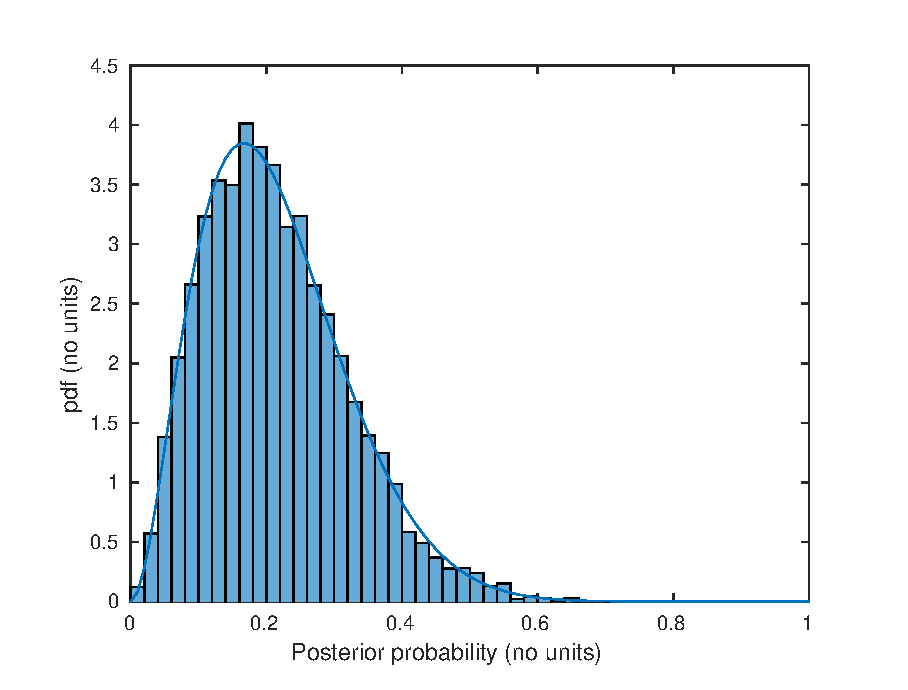
\includegraphics[width=0.5\textwidth]{binomial_ABC0528.eps}
\caption{Histogram of 10,000 samples of $\textup{Beta}(3,11)$ using ABC. The curve shows the exact posterior distribution function. The $p$-value for the $\chi^2$ goodness of fit test in this example was $5\%$ to one significant figure.}
\label{binomial}
\end{figure}

\section{Normal-Gamma prior, Normal likelihood}

\subsection{Method}
Suppose the parameters $\theta$ and $\tau$ have a prior distribution such that
\begin{equation}
\tau\sim\textup{Gamma}(\alpha_0,\beta_0)
\end{equation}
and
\begin{equation}
\mu|\tau\sim\textup{N}\left(\mu_0,1/(\nu_0\tau)\right) \ .
\end{equation}
In other words, the joint prior distribution is such that
\begin{equation}
\mu,\tau\sim\textup{NGamma}(\mu_0,\nu_0,\alpha_0,\beta_0) \ .
\end{equation}
Let a random variable $X$ given the prior be distributed such that
\begin{equation}
X|\mu,\tau\sim\textup{N}(\mu,1/\tau) \ .
\end{equation}

After observing $n$ samples of $X$, labelled $x_1,x_2,\dotdotdot ,x_n$, the joint posterior distribution is given as
\begin{equation}
(\mu,\tau|X=\{x_1,\dotdotdot ,x_n\})\sim\textup{NGamma}
\left(
	\mu_1,
	\nu_1,
	\alpha_1,
	\beta_1
\right) \ .
\end{equation}
where the posterior parameters are
\begin{align}
\mu_1 &= \dfrac{n\bar{x}+\nu_0\mu_0}{n+\nu_0} \\
\nu_1 &= n+\nu_0 \\
\alpha_1 &= \dfrac{n}{2}+\alpha_0 \\
\beta_1 &= \beta_0+\dfrac{S_{xx}}{2}+\dfrac{n\nu_0(\bar{x}-\mu_0)^2}{2(n+\nu_0)} \ ,
\end{align}
$S_{xx}$ is the sum of squared difference from the sample mean and $\bar{x}$ is the sample mean.

The marginal posterior distribution is given as
\begin{equation}
(\mu|X=\{x_1,\dotdotdot ,x_n\}) = \sqrt{\dfrac{\beta_1}{\alpha_1\nu_1}} T_{2\alpha_1}
+ \mu_1
\end{equation}
and
\begin{equation}
(\tau|X=\{x_1,\dotdotdot ,x_n\}) \sim \textup{Gamma}\left(
\alpha_1,\beta_1
\right)
\end{equation}
where $T_{2\alpha}\sim t_{2\alpha}$.

ABC can be used to sample the posterior distribution but only approximately due to the arbitrary choice of comparing two samples of continuous random variables. Here, the observed and simulated samples from ABC were compared by means of hypothesis testing on the sample mean and sample standard deviation. That is, the posterior accept/reject sampling scheme is as followed:
\begin{itemize}
	\item Sample $\tau\sim\textup{Gamma}(\alpha_0,\beta_0)$
	\item Sample $\mu|\tau\sim\textup{N}\left(\mu_0,1/(\nu_0\tau)\right)$
	\item Sample $n$ times $Y|\mu,\tau\sim\textup{N}(\mu,1/\tau)$
	\item Conduct two tailed hypothesis tests, at some confidence level, on
	\begin{equation}
	\dfrac{\sqrt{n}\left(\bar{X}-\bar{Y}\right)}{\sqrt{S_X^2+S_Y^2}}\sim\textup{N}(0,1)
	\end{equation}
	\begin{equation}
	\dfrac{S_X^2}{S_Y^2}\sim F_{n-1,n-1}
	\end{equation}
	\item Accept $\mu,\tau$ if both null hypothesis are accepted, reject otherwise
\end{itemize}
where $\bar{X}$ and $S_X^2$ are the sample mean and sample variance of the observed $X$ respectively. Similarly $\bar{Y}$ and $S_Y^2$ are the sample mean and sample variance of the simulated $Y$.

\subsection{Results}
The prior parameters were set to be $\mu_0=1,\nu_0=2,\alpha_0=2,\beta_0=1$. Samples of $X$ were observed by simulating $n=10$ samples from the standard Normal distribution.

1000 posterior samples were drawn using ABC with different confidence levels for the hypothesis tests. Figure \ref{surf} shows the joint histogram of the posterior samples, using a confidence level of $10\%$, compared with the true posterior distribution. By inspection, it appeared that samples from ABC is a good approximation to the posterior distribution.

The $\chi^2$ goodness of fit test was conducted on the marginal samples of the posterior distribution, as shown in Figures \ref{mean} and \ref{precision}. The $p$ values for the goodness of fit test were obtained 50 times using different observations of $X$ for different confidence levels as shown in Figures \ref{pvalue_mean} and \ref{pvalue_precision}. From the figures, there is a general trend that the $p$ values increases for smaller confidence levels as expected. However the $p$ values for confidence levels $10\%$ and $20\%$ were very similar, thus there was not much improvement in the goodness of fit test when decreasing the confidence level to $10\%.$

Figure \ref{rejections} shows the number of rejections per accepted sample when using ABC. As expected, the number of rejections increased for smaller confidence levels. However the number of rejections increased, from $(80\pm80)$ to $(1000\pm1000)$, when decreasing the confidence level from $20\%$ to $10\%$. This is an increase in the order of $10^2$.

In conclusion, a confidence level of $20\%$ is good enough for ABC to approximately sample the posterior distribution. While a confidence level of $10\%$ should give a more accurate result, it suffers from very high rejection rates.

\begin{figure}
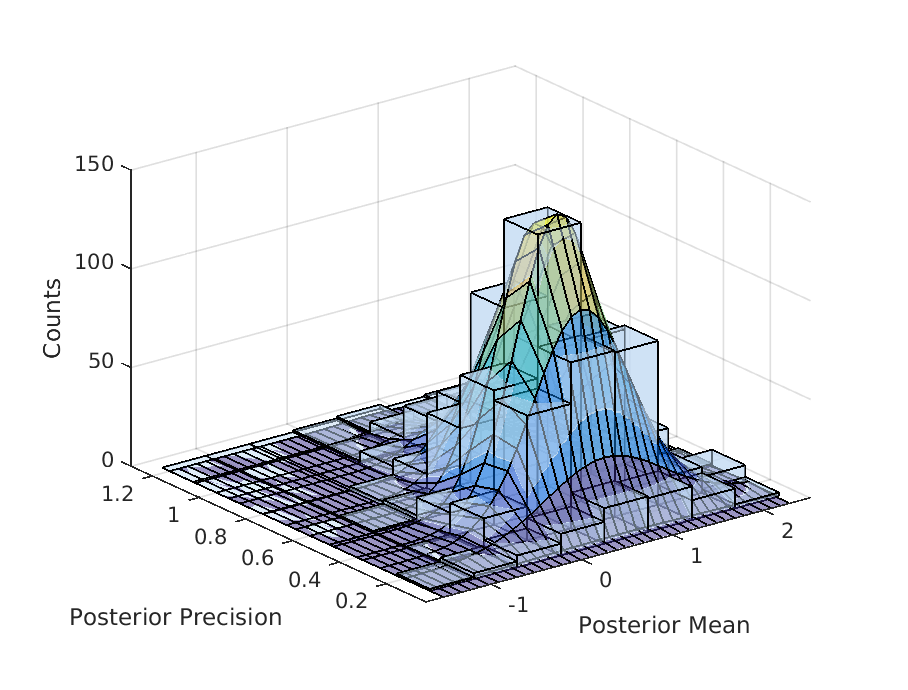
\includegraphics[width=0.5\textwidth]{surf.eps}
\caption{Joint histogram of 1000 samples of the posterior distribution using ABC compared with the true joint posterior distribution, shown as a surface plot. The confidence level was set at $10\%$ for the ABC accept/reject sampling scheme.}
\label{surf}
\end{figure}

\begin{figure}
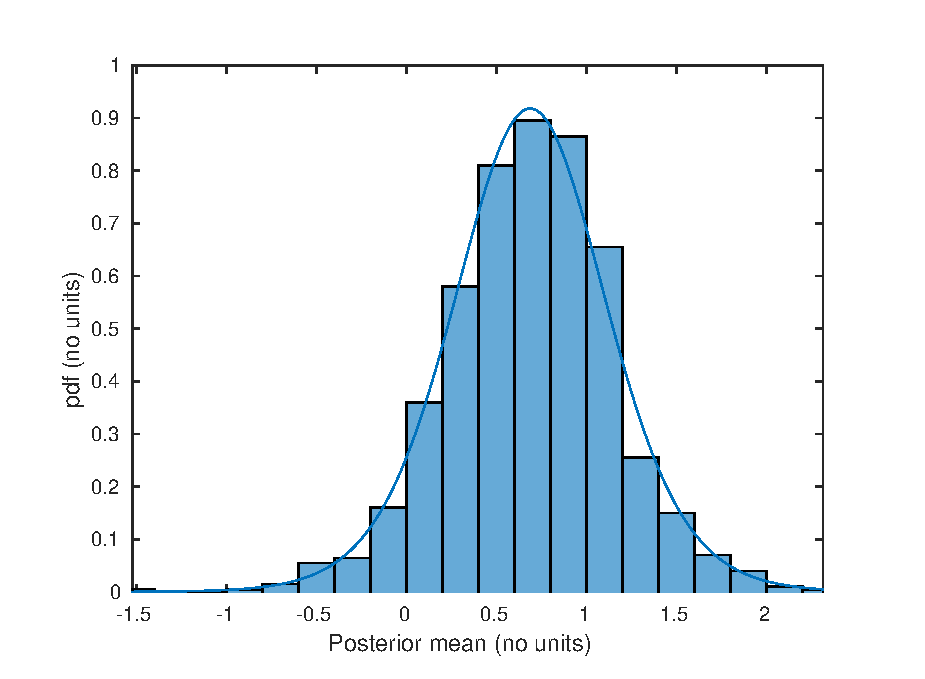
\includegraphics[width=0.5\textwidth]{mean.eps}
\caption{Marginal histogram of 1000 samples of the posterior mean, using ABC, compared with the true marginal posterior distribution. The confidence level was set at $10\%$ for the ABC accept/reject sampling scheme. In this example, the $p$ value for the $\chi^2$ goodness of fit test was $60\%$ to one significant figure.}
\label{mean}
\end{figure}

\begin{figure}
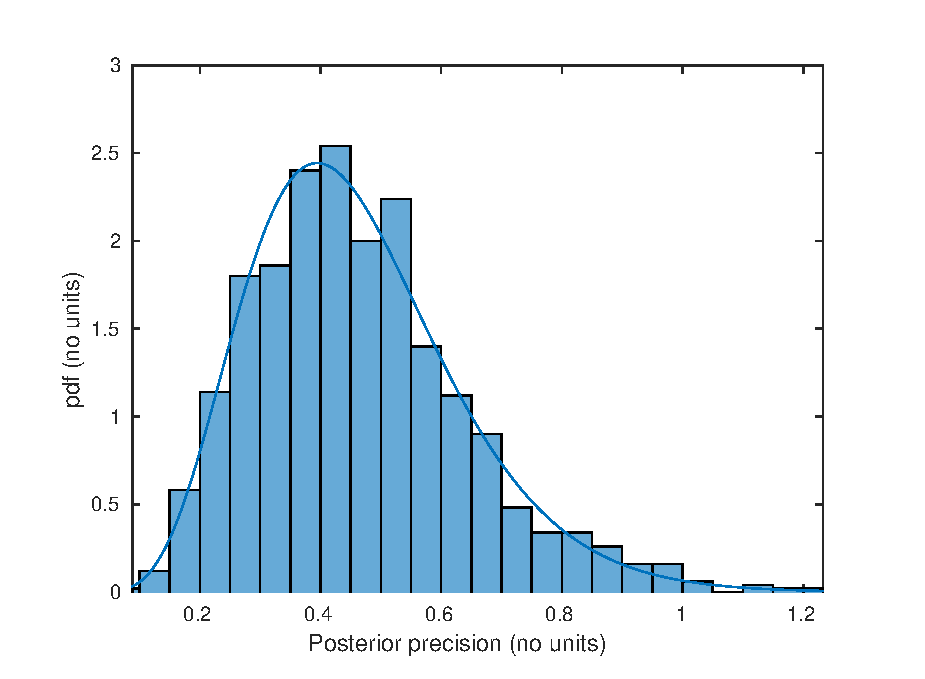
\includegraphics[width=0.5\textwidth]{precision.eps}
\caption{Marginal histogram of 1000 samples of the posterior precision, using ABC, compared with the true marginal posterior distribution. The confidence level was set at $10\%$ for the ABC accept/reject sampling scheme. In this example, the $p$ value for the $\chi^2$ goodness of fit test was $30\%$ to one significant figure.}
\label{precision}
\end{figure}

\begin{figure}
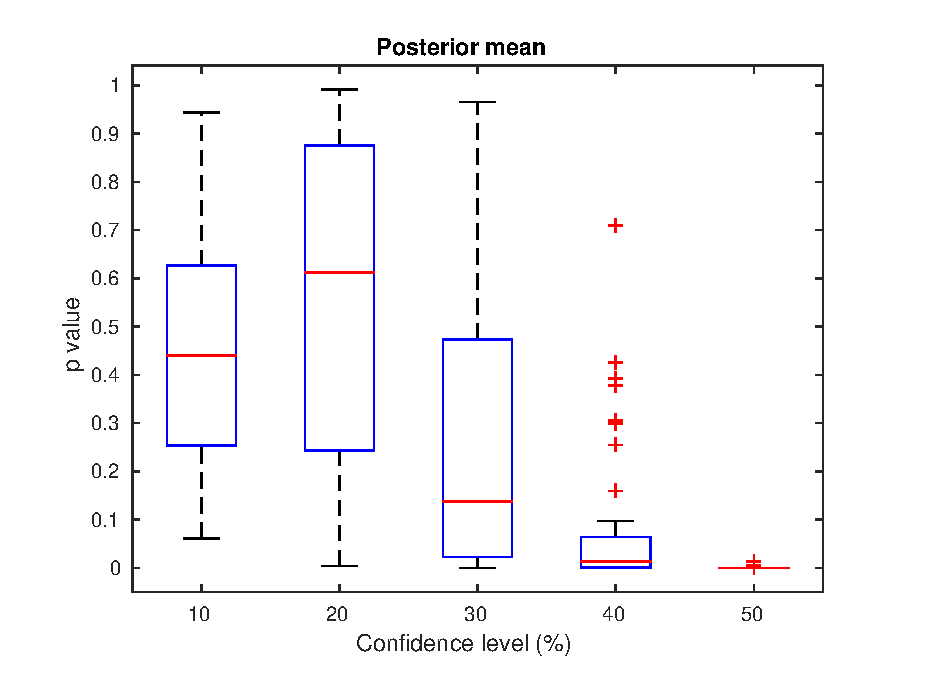
\includegraphics[width=0.5\textwidth]{pvalue_mean.eps}
\caption{$p$ values for the $\chi^2$ goodness of fit test on the marginal samples of the posterior mean. For each confidence level, fifty $p$ values were obtained by repeating the test using different observations of the random variable $X$.}
\label{pvalue_mean}
\end{figure}

\begin{figure}
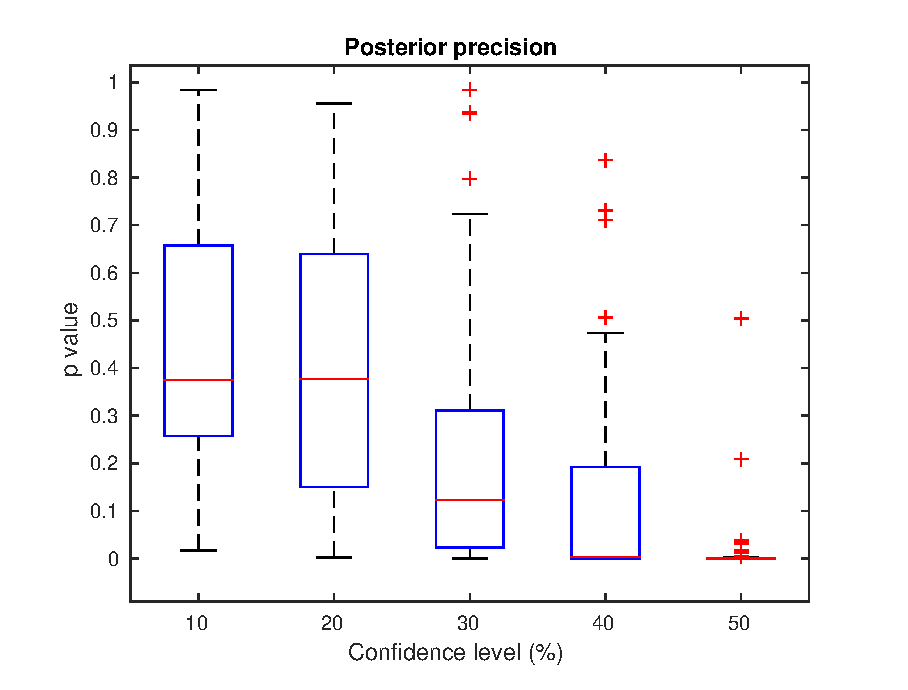
\includegraphics[width=0.5\textwidth]{pvalue_precision.eps}
\caption{$p$ values for the $\chi^2$ goodness of fit test on the marginal samples of the posterior precision. For each confidence level, fifty $p$ values were obtained by repeating the test using different observations of the random variable $X$.}
\label{pvalue_precision}
\end{figure}

\begin{figure}
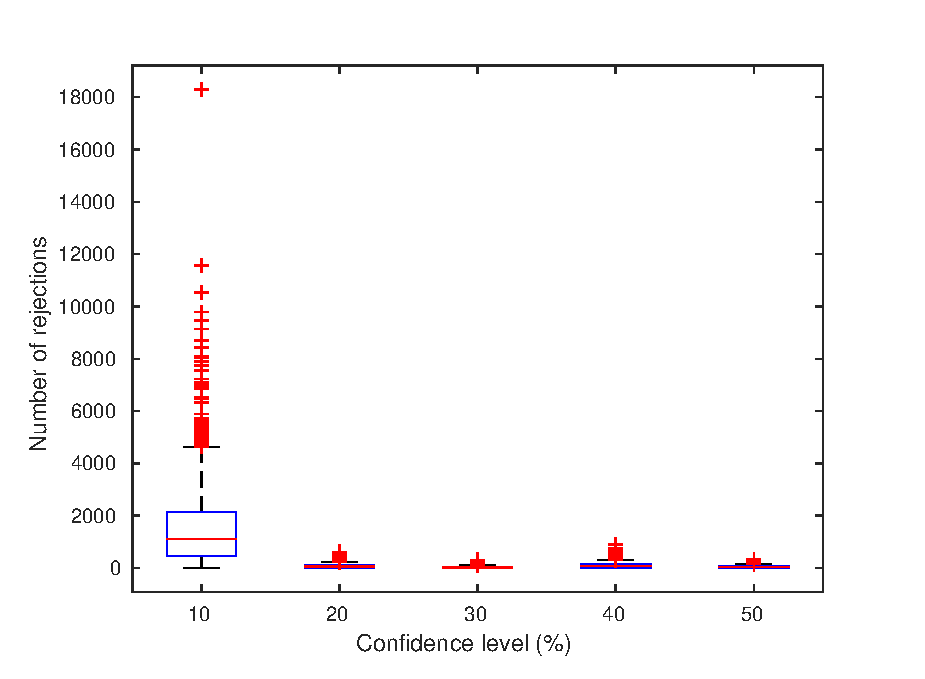
\includegraphics[width=0.5\textwidth]{rejections.eps}
\caption{The number of rejected samples per accepted sample using ABC.}
\label{rejections}
\end{figure}

\section{Conclusion}
It was found that in these ABC experiments, ABC does approximate the posterior distribution well but can suffer from high rejection rates. A good confidence level, or threshold, is one which is small enough that samples, drawn from ABC, approximates the posterior distribution well but big enough the rejection rate is feasible.

The hypothesis tests used were chosen so that comparison of two samples was done only through minimal sufficient statistics. It should be noted that for more complicated models the sufficient statistics for each parameter may not be known.

When the posterior distribution is not known, then there is no way to tell how well ABC approximates the posterior. The threshold can be set as small as possible to minimize error, however high rejection rates will happen especially if the prior distribution is very different to the posterior distribution.

It should also be noted that improper priors cannot be simulated thus cannot be used for ABC in this context.


% \subsection{Method}
% Suppose a parameter $\theta$ has a prior distribution such that
% \begin{equation}
% \theta\sim\textup{Beta}(1,1)
% \end{equation}
% and that a random variable $X$ is distributed such that
% \begin{equation}
% X|\theta\sim\textup{Bin}(12,\theta) \ .
% \end{equation}
% Then after observing $X=2$, the posterior distribution is given as
% \begin{equation}
% (\theta|X=2)\sim\textup{Beta}(3,11) \ .
% \end{equation}
% ABC was used to sample the posterior distribution where the algorithm is as followed:
% \begin{itemize}
%   \item Sample $\theta$ from the uniform distribution
%   \item Sample $X|\theta$ from the likelihood
%   \item If the sampled $X|\theta$ is equal to 2, accept $\theta$, otherwise reject.
% \end{itemize}

% \subsection{Results}
% 10,000 posterior samples were drawn from the ABC algorithm. These were compared with the true posterior distribution, as shown in Figure \ref{binomial}, using the $\chi^2$ goodness of fit test.  By repeating the experiment 50 times, the mean and standard deviation $p$-value for the $\chi^2$ test was found to be $(50\pm30)\%$. This is very strong evidence that the ABC posterior samples do estimate the posterior distribution well.

% The mean and standard deviation number of rejected samples per accepted sample was estimated to $(10\pm10)$.

% \begin{figure}
% 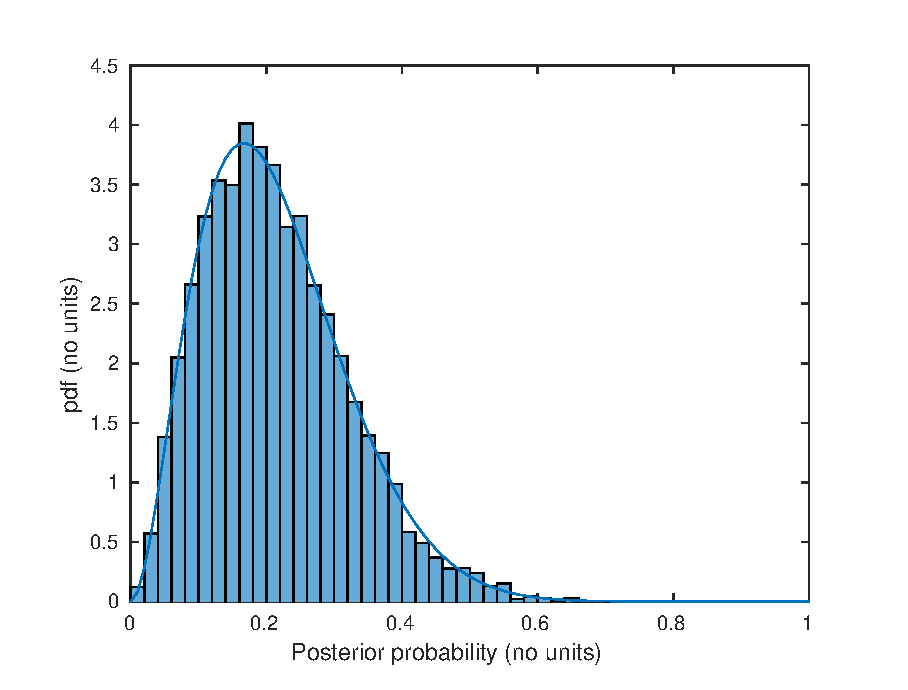
\includegraphics[width=0.5\textwidth]{binomial_ABC0528.eps}
% \caption{Histogram of 10,000 posterior samples of $\textup{Beta}(3,11)$ using ABC. The curve shows the exact posterior distribution function. The $p$-value for the $\chi^2$ goodness of fit test in this example was $5\%$ to one significant figure.}
% \label{binomial}
% \end{figure}

% \section{Normal-Gamma prior, Normal likelihood}

% \subsection{Method}
% Suppose the parameters $\theta$ and $\tau$ have a prior distribution such that
% \begin{equation}
% \tau\sim\textup{Gamma}(\alpha_0,\beta_0)
% \end{equation}
% and
% \begin{equation}
% \mu|\tau\sim\textup{N}\left(\mu_0,1/(\nu_0\tau)\right) \ .
% \end{equation}
% In other words, the joint prior distribution is such that
% \begin{equation}
% \mu,\tau\sim\textup{NGamma}(\mu_0,\nu_0,\alpha_0,\beta_0) \ .
% \end{equation}
% Let a random variable $X$ given the prior be distributed such that
% \begin{equation}
% X|\mu,\tau\sim\textup{N}(\mu,1/\tau) \ .
% \end{equation}

% After observing $n$ samples of $X$, labelled $x_1,x_2,\dotdotdot ,x_n$, the joint posterior distribution is given as
% \begin{multline}
% (\mu,\tau|X=\{x_1,\dotdotdot ,x_n\})\sim\textup{NGamma}
% \left(
% 	\mu_1,
% 	\right.\\\left.
% 	\nu_1,
% 	\alpha_1,
% 	\beta_1
% \right) \ .
% \end{multline}
% where the posterior parameters are
% \begin{align}
% \mu_1 &= \dfrac{n\bar{x}+\nu_0\mu_0}{n+\nu_0} \\
% \nu_1 &= n+\nu_0 \\
% \alpha_1 &= \dfrac{n}{2}+\alpha_0 \\
% \beta_1 &= \beta_0+\dfrac{S_{xx}}{2}+\dfrac{n\nu_0(\bar{x}-\mu_0)^2}{2(n+\nu_0)} \ ,
% \end{align}
% $S_{xx}$ is the sum of squared difference from the mean and $\bar{x}$ is the sample mean.

% The marginal posterior distribution is given as
% \begin{equation}
% (\mu|X=\{x_1,\dotdotdot ,x_n\}) = \sqrt{\dfrac{\beta_1}{\alpha_1\nu_1}} T_{2\alpha_1}
% + \mu_1
% \end{equation}
% and
% \begin{multline}
% (\tau|X=\{x_1,\dotdotdot ,x_n\}) \sim \textup{Gamma}\left(
% \alpha_1,\beta_1
% \right)
% \end{multline}
% where $T_{2\alpha}\sim t_{2\alpha}$.

% ABC can be used to sample the posterior distribution but only approximately due to the arbitrary choice of comparing two samples of continuous random variables. Here, the observed and simulated samples from ABC were compared by means of hypothesis testing on the sample mean and sample standard deviation. That is, the the posterior accept/reject sampling scheme is as followed:
% \begin{itemize}
% 	\item Sample $\tau\sim\textup{Gamma}(\alpha_0,\beta_0)$
% 	\item Sample $\mu|\tau\sim\textup{N}\left(\mu_0,1/(\nu_0\tau)\right)$
% 	\item Sample $n$ times $Y|\mu,\tau\sim\textup{N}(\mu,1/\tau)$
% 	\item Conduct two tailed hypothesis tests, at some confidence level $\epsilon$, on
% 	\begin{equation}
% 	\dfrac{\sqrt{n}\left(\bar{X}-\bar{Y}\right)}{\sqrt{S_X^2+S_Y^2}}\sim\textup{N}(0,1)
% 	\end{equation}
% 	\begin{equation}
% 	\dfrac{S_X^2}{S_Y^2}\sim F_{n-1,n-1}
% 	\end{equation}
% 	\item Accept $\mu,\tau$ if both null hypothesis are accepted, reject otherwise
% \end{itemize}
% where $\bar{X}$ is the sample mean and $S_X^2$ is the sample standard deviation.

% \subsection{Results}
% The prior parameters were set to be $\mu_0=1,\nu_0=2,\alpha_0=2,\beta_0=1$. Samples of $X$ were observed by simulating $n=10$ samples from the standard Normal distribution.

% 1000 posterior samples were drawn using ABC with different confidence levels for the hypothesis tests. Figure \ref{surf} shows the joint histogram of the posterior samples compared with the true posterior distribution, using a confidence level of $10\%$. By inspection, it appeared that samples from ABC is a good approximation to the posterior distribution.

% The $\chi^2$ goodness of fit test was conducted on the marginal samples of the marginal posterior distribution, as shown in Figures \ref{mean} and \ref{precision}. The $p$ values for the goodness of fit test were obtained 50 times using different observations of $X$ for different confidence levels as shown in Figures \ref{pvalue_mean} and \ref{pvalue_precision}. From the figures, there is a general trend that the $p$ values increases for smaller confidence levels as expected. However the $p$ values for confidence levels $10\%$ and $20\%$ were very similar, thus there was not much improvement in the goodness of fit test when decreasing the confidence level to $10\%.$

% Figure \ref{rejections} shows the number of rejections per accepted sample when using ABC. As expected, the number of rejections increases for larger confidence levels. However the magnitude of the number of rejections increased by an order of $10^2$ when decreasing the confidence level from  $20\%$ to $10\%$.

% In conclusion, a confidence level of $20\%$ is good enough for ABC to approximately sample the posterior distribution. While a confidence level of $10\%$ should give a more accurate result, it suffers from very high rejection rates.

% \begin{figure}
% 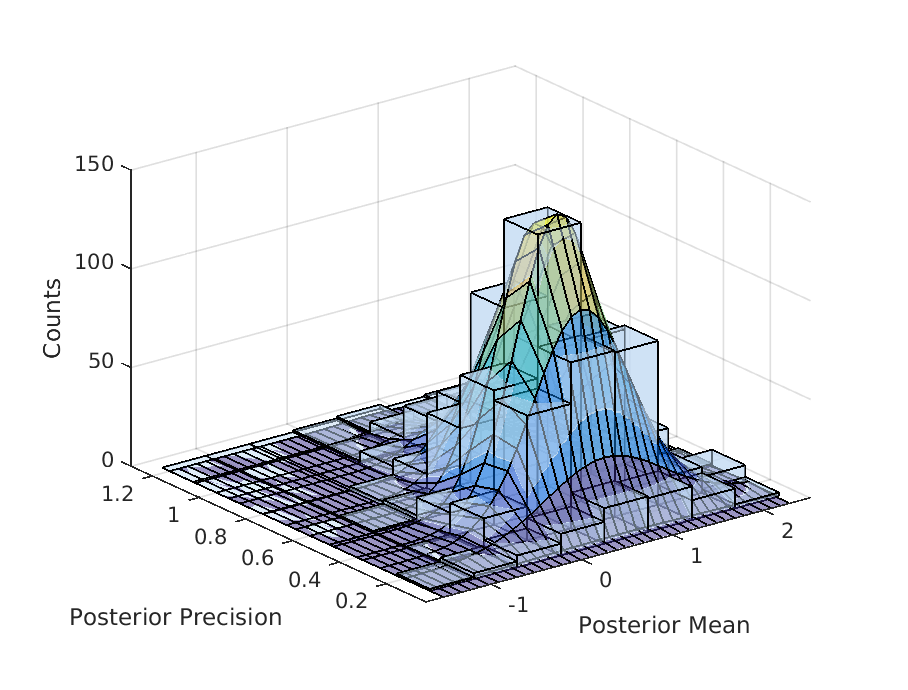
\includegraphics[width=0.5\textwidth]{surf.eps}
% \caption{Joint histogram of samples of the posterior distribution using ABC compared with the true joint posterior distribution, shown as a surface plot. The confidence level was set at $10\%$ for the ABC accept/reject sampling scheme.}
% \label{surf}
% \end{figure}

% \begin{figure}
% 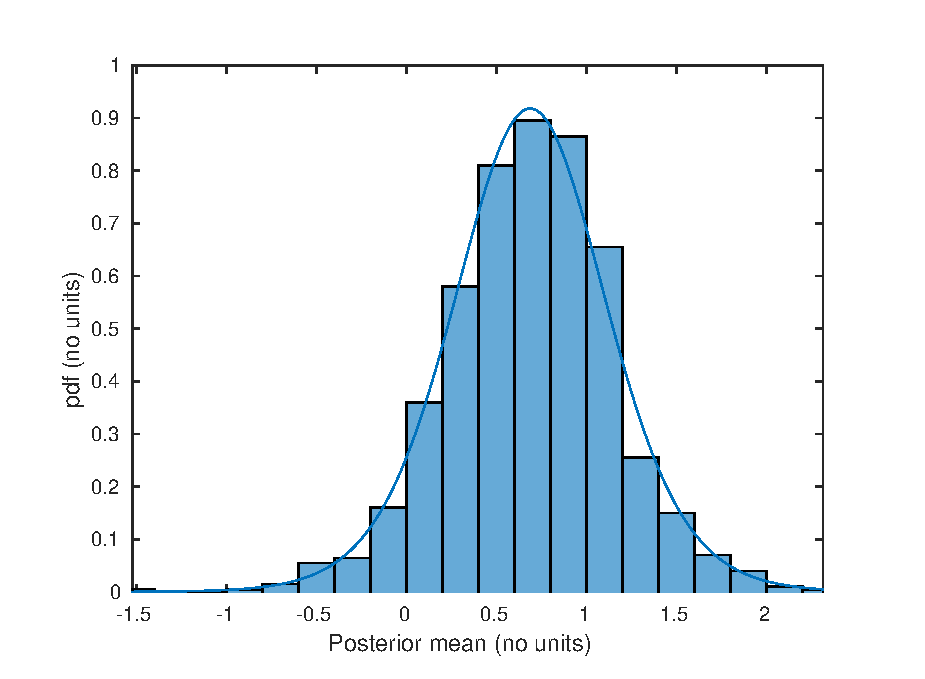
\includegraphics[width=0.5\textwidth]{mean.eps}
% \caption{Marginal histogram of samples of the posterior mean, using ABC, compared with the true marginal posterior distribution. In this example, the $p$ value for the $\chi^2$ goodness of fit test was $60\%$ to one significant figure.}
% \label{mean}
% \end{figure}

% \begin{figure}
% 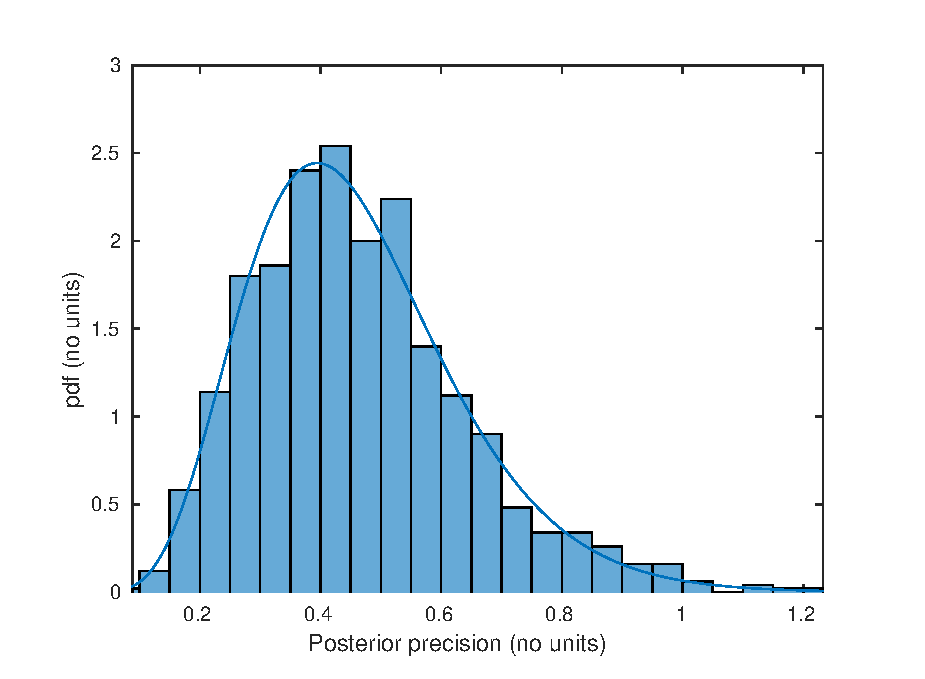
\includegraphics[width=0.5\textwidth]{precision.eps}
% \caption{Marginal histogram of samples of the posterior precision, using ABC, compared with the true marginal posterior distribution. In this example, the $p$ value for the $\chi^2$ goodness of fit test was $30\%$ to one significant figure.}
% \label{precision}
% \end{figure}

% \begin{figure}
% 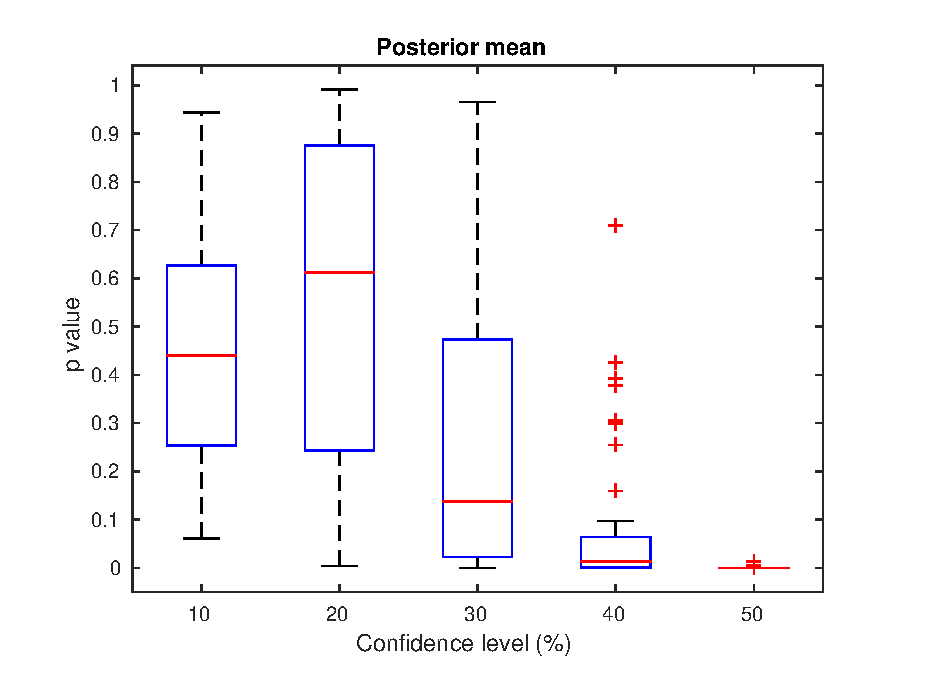
\includegraphics[width=0.5\textwidth]{pvalue_mean.eps}
% \caption{$p$ values for the $\chi^2$ goodness of fit test on the marginal samples of the posterior mean. For different confidence levels, fifty $p$ values were obtained by repeating the test using different observations of the random variable $X$.}
% \label{pvalue_mean}
% \end{figure}

% \begin{figure}
% 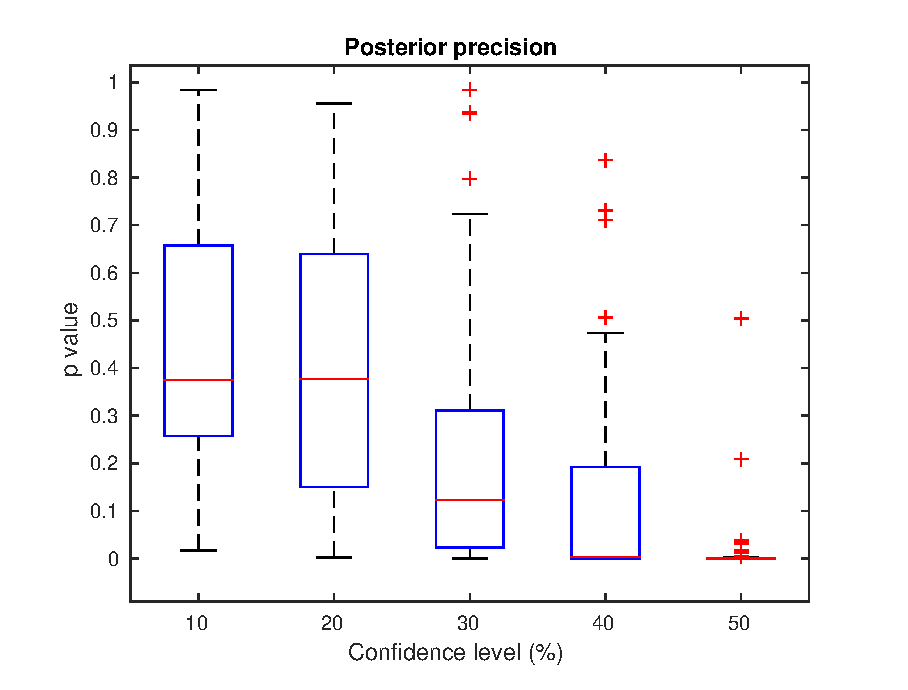
\includegraphics[width=0.5\textwidth]{pvalue_precision.eps}
% \caption{$p$ values for the $\chi^2$ goodness of fit test on the marginal samples of the posterior precision. For different confidence levels, fifty $p$ values were obtained by repeating the test using different observations of the random variable $X$.}
% \label{pvalue_precision}
% \end{figure}

% \begin{figure}
% 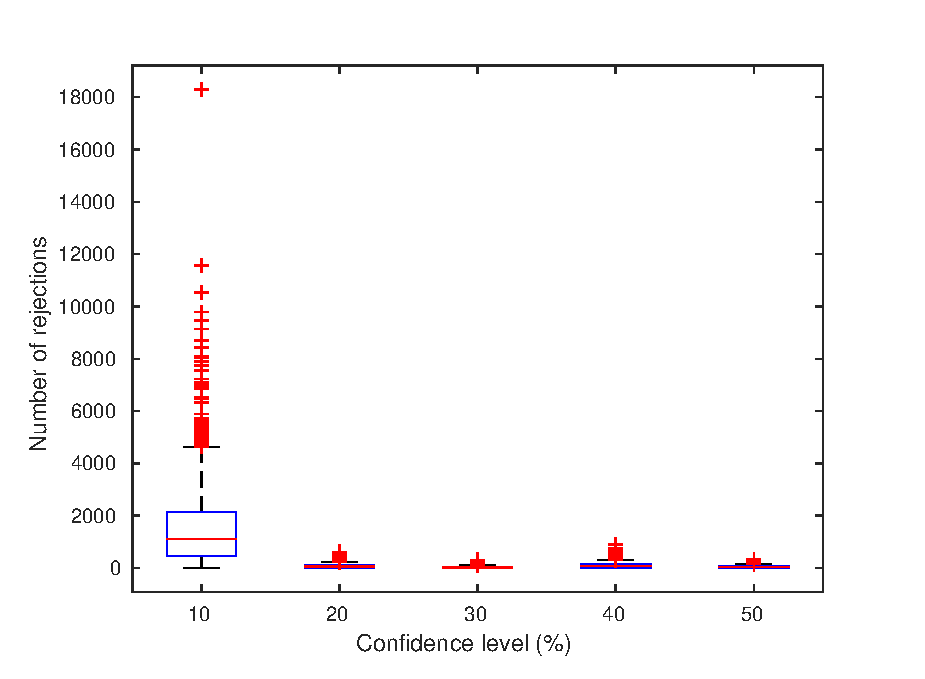
\includegraphics[width=0.5\textwidth]{rejections.eps}
% \caption{The number of rejection samples per accepted sample using ABC.}
% \label{rejections}
% \end{figure}

% \section{Evaluation}
% It was found that in these ABC experiments, ABC does approximate the posterior distribution well but can suffer from high rejection rates. A good threshold is one which is small enough that samples from ABC approximate the posterior distribution well but big enough the rejection rate is feasible. It should also be noted that improper priors cannot be simulated thus cannot be used for ABC.

% When the posterior distribution is not known, then there is no way to tell how well ABC approximates the posterior. The threshold can be set as small as possible, however high rejection rates will happen, especially if the prior distribution is very different to the posterior distribution.
% % \bibliography{Module2bib}

\section{Conclusions}
Many more sophisticated versions of ABC.

\end{document}

\begin{figure}[h] 
\centering
\includegraphics[width=0.6\textwidth]{graph_nd.pdf}
\caption{The Chen-Stein bounds on the distance between $\mathbb{P}(W=0)$ and $\mathbb{P}(Z=0)$ as $n$ increases, keeping the ratio $\frac{n^k}{d^{1-k}}$ constant at 1.45.}
\label{fig:graph_nd}
\end{figure}